\chapter{Experiments}\label{chap:experiments}

In this chapter, we will be providing more graphic material for the different models detailed in chapter \ref{chap:methods}.
We will be going over the three models and their experiments again, providing extra results that were not shown earlier.

\section{First model: CNN speed regressor}\label{sec:speed_regression_model}

This model is a deep CNN that predicts the average velocity norm (i.e. speed) of a unit from a window of IMU measurements. 
We test this model on the inertial data of the EuRoC dataset, which we found is extremely corrupted by vibration noise, making the learning task much difficult. 
We remove the noise using the filtering technique specified in the Appendix section \ref{sec:euroc_filtering}, and after 150 epochs we manage to fit in the training set.
Furthermore, we do some normalization preprocessing of the IMU input data, which we also found was necessary to fit the model.
Without these two requirements, the architecture was not able to make sense of the data.

Figure \ref{fig:speed_prediction_filtered_vs_unfiltered} shows the results of our predictions on the training set. 
On the left plot, noise has been removed from the dataset using the low-pass filtering. 
Notice how the predictions on the left image (unfiltered data) during the first 5000 samples are as nearly as accurate as in the filtered counterpart.
This is because during the first seconds of the flight, the drone is moved by hand, and therefore there is no vibration noise.
We can however see that, in the presence of high frequency noise, the predictions are much less accurate.

\begin{figure}[h]
   \centering
   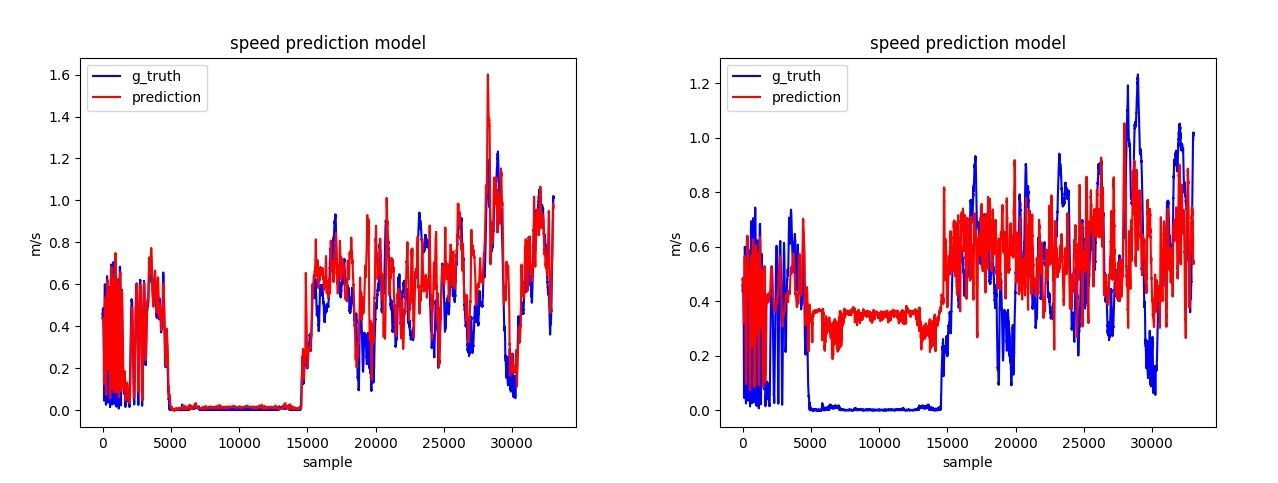
\includegraphics[width=0.95\textwidth]{thesis_template/img/speed_prediction_filtered_vs_unfiltered.jpeg}
   \caption{Linear speed regression in the EuRoC training set, with (left) and without (right) the dataset pre-processing specified in appendix Section \ref{sec:euroc_filtering}.
   The regressor is not able to fit the training data when the IMU noise is not filtered out.}
   \label{fig:speed_prediction_filtered_vs_unfiltered}
\end{figure}

Furthermore, Figure \ref{fig:speed_prediction_filtered_vs_unfiltered_validation} shows the same experiment than Figure \ref{fig:speed_prediction_filtered_vs_unfiltered} but evaluated on a separate held-out test set not used during training.
In this case, the model cannot properly predict any of the two datasets, but on top of that the predictions oscillate more in the unfiltered case.

\begin{figure}[h]
   \centering
   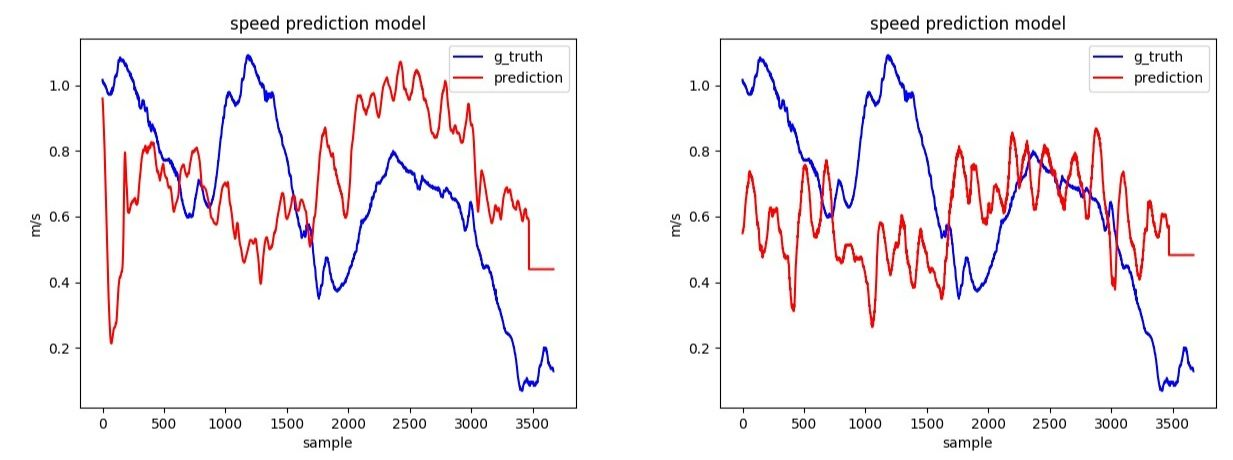
\includegraphics[width=0.95\textwidth]{thesis_template/img/speed_prediction_validation_filtered_vs_unfiltered.jpeg}
   \caption{Linear speed regression in the EuRoC held-out validation set, with (left) and without (right) the dataset pre-processing specified in appendix Section \ref{sec:euroc_filtering}.
   The regressor is not able to properly predict the correct speed values from the ground truth, but the predictions are even less accurate without the filtering.}
   \label{fig:speed_prediction_filtered_vs_unfiltered_validation}
\end{figure}

To evaluate the efficacy of our filtering strategy, we apply it to an ideal EuRoC dataset, generated with a Visual-Inertial simulator from Zurich eye. 
This dataset is completely free of IMU noise, and has been generated from the flight sequence "Machine Hall 1", which was not used to train our model, so we consider it as a valid test set.
We use once again our model to regress the linear speed across time (see Figure \ref{fig:speed_prediction_filtered_vs_unfiltered_ideal}).
The predictions of the model are not very accurate, but it appears like the model has indeed learned something about how to estimate the speed of the drone.
We also perform a sanity check by predicting on an unfiltered version of this ideal dataset, and verify that the predictions very similar than with the filtered data (right plot).
This means that, as we hypothesize in Section \ref{sec:euroc_filtering}, the low frequencies (smaller than 10Hz) contain nearly all the relevant information for the state estimation task, and the higher ones can be removed quite safely.

\begin{figure}[h]
   \centering
   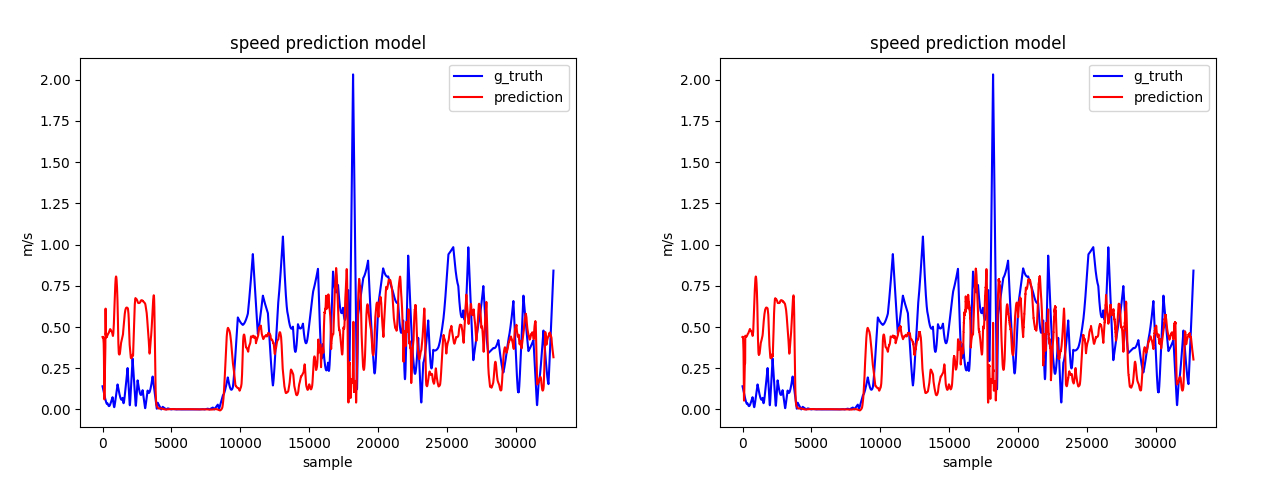
\includegraphics[width=0.95\textwidth]{thesis_template/img/speed_prediction_ideal_filtered_vs_unfiltered.jpg}
   \caption{
   Linear speed regression in an ideal, noiseless, EuRoC test set, with (left) and without (right) the dataset pre-processing specified in appendix Section \ref{sec:euroc_filtering}.
   Both predictions look almost identical, which confirms that the low-frequency components of the IMU signal contain the most relevant information needed by the model to regress the speed norm value.}
   \label{fig:speed_prediction_filtered_vs_unfiltered_ideal}
\end{figure}

\section{Second model: IMU state integrator}

This second model aims at reproducing IMU integration with a deep model. 
Of course, one important requirement is that the model should learn how the noise and bias of the inertial sensor work, so that it can remove them intrinsically as much as possible.
We do this by using as training set the noiseless ground truth data as target.
To evaluate the performance of the trained models for this task, we design two different experiments that evaluate their short-term and long-term reliability. 

The first experiment, which we call the \emph{one-step} experiment, inputs to the models a starting state $\mathbf{x}(k-w)\in\mathbb{R}^{10}$ together with $w$ IMU measurements from sample $k-w$ until $k$: $\mathbf{\hat{M}}_k\in\mathbb{R}^{w\times6}$ and expects to receive the output state $\mathbf{\hat{x}}(k)$, which is compared with the corresponding ground truth measurement $\mathbf{x}(k)$.
This experiment is used safety check, as normally the system state estimate is not expected to drift significantly because of noise in just $w$ samples.

Once the model passes the first experiment, the second one is performed, which we call the \emph{iterative} experiment.
In this case, an initial state $\mathbf{x}(0)$ is given to the system, together with a succession of n windows of IMU measurements: $\left(\mathbf{\hat{M}}_w,\mathbf{\hat{M}}_{2w},...,\mathbf{\hat{M}}_{nw}\right)$, with overlap in just the last sample (i.e. overlap 1). 
The system must use all the inputs to generate a sequence of predictions $\left(\mathbf{\hat{x}}_w, ..., \mathbf{\hat{x}}_{nw}\right)$, using the intermediate predictions its own state input for next iteration.

\subsection{First model iteration: $\mathbf{x}(k),\; \mathbf{\hat{x}}(k)\in\mathbb{R}^{10}$}
For the first iteration of this model, we train the architecture described in Figure \ref{fig:state_int_v0}, where the output state is a 10-dimensional vector containing the predicted position, velocity and rotation, in unit quaternion form. 
As a proof of concept, we train this model on a rather flat flight from the BB dataset (\emph{Thrice}), and with a maximum speed of 2m/s, which is also quite slow. 

We then test the model on a second flight sequence (\emph{bentDice}, $v_{max}=2m/s$), which is actually rich in 3D motion.
We perform first the one-set integration test against this test set. 
As we showed in Figure \ref{fig:imu_int_50} in last section, the model is quite reasonably able to predict the position x and y, and the speed of the drone also in these two axes. 
However, it fails to properly calculate the rotation, or the z component of $\mathbf{p}$ and $\mathbf{v}$. 
Figure \ref{fig:imu_int_50_r10_3d} provides a 3D visualization of the position vector, where we can see that the predicted positions are not particularly better than IMU integration for most of the trajectory.

\begin{figure}[h]
   \centering
   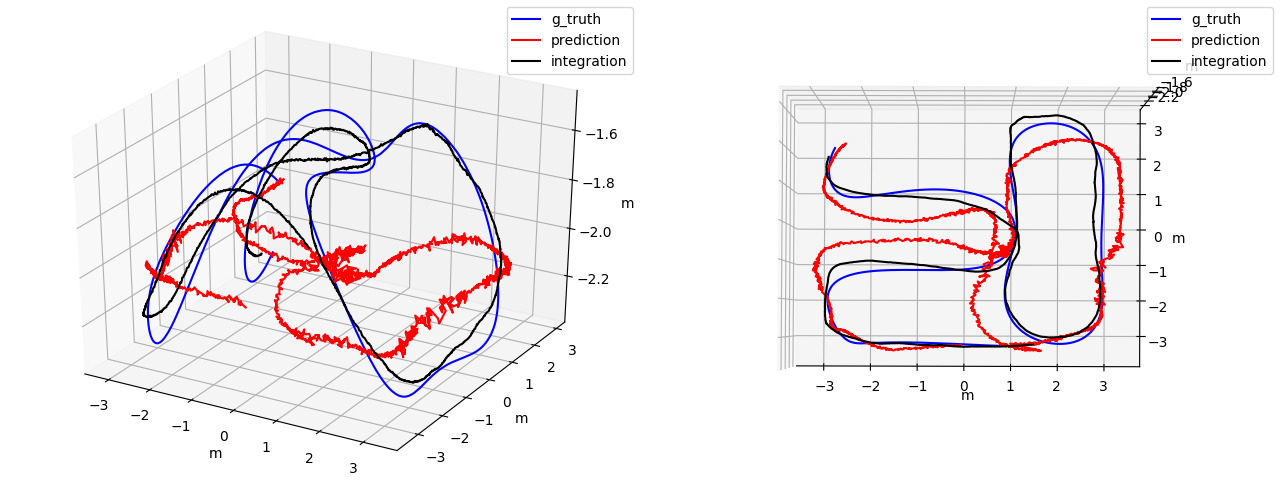
\includegraphics[width=0.85\textwidth]{thesis_template/img/imu_int_50_3d.jpg}
   \caption{3D visualization of the position ground truth, compared with the model predictions and IMU double integration algorithm. 
   3D view (left) vs top view (right). The model under-performs double-integration in all three dimensions, especially in the z axis, because the training data was planar and the model could not learn motion in this dimension.}
   \label{fig:imu_int_50_r10_3d}
\end{figure}

\subsection{Second model iteration: $\mathbf{x}(k)\in\mathbb{R}^{10},\; \mathbf{\hat{x}}(k)\in\mathbb{R}^{9}$}\label{sec:exp_imu_int_so3}

While z-dimension problem in the previous approach is expected, since the original training set of the model was a quite flat flight, we hypothesize that the rotation problem is due to the high non-linearity of the quaternion loss term (described in \ref{eq:q_state_loss}).
To fix this, we change the output format of the model, so that the predicted rotation component is in Lie algebra, which allows to use MSE loss \ref{eq:state_so3_loss} instead of the highly nonlinear quaternion angle loss.
An exponential mapping can then be applied to remap this rotation component back to quaternion form.

This new approach is retrained, this time on the 3D \emph{bentDice} dataset, also with a maximum speed of 2m/s.
Then, the one-step integration experiment is repeated on a split test set of the same flight sequence, which yields the results in Figure \ref{fig:imu_so3_bentdice_val}, where it is evident that the fit of the $\boldsymbol{\mathfrak{q}}$ rotation vector is much better than in Figure \ref{fig:imu_int_50}.

\begin{figure}[h]
   \centering
   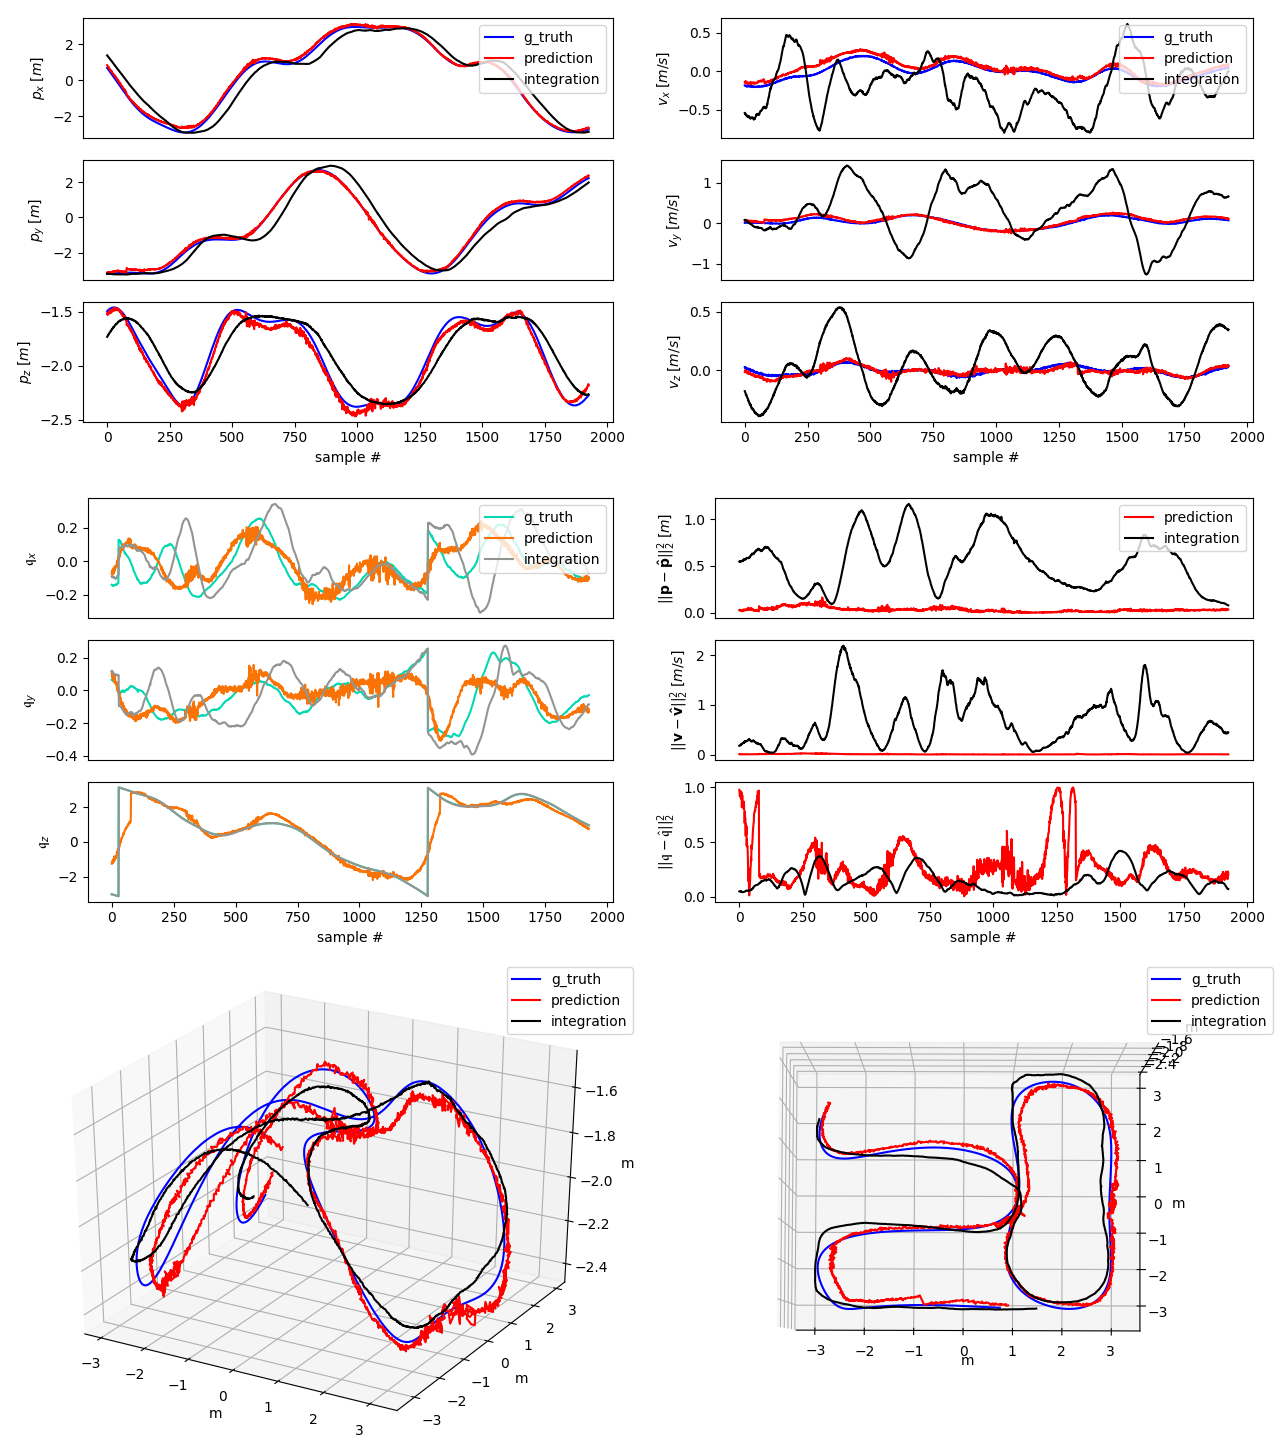
\includegraphics[width=0.85\textwidth]{thesis_template/img/imu_int_50_so3_bentDice_validation_full.jpg}
   \caption{Results of the $\mathfrak{so}(3)$ based model on a split test set from the \emph{bentDice} sequence compared with ground truth and IMU double integration. From left to right, and top to bottom, the plots represent: $\mathbf{p}$, $\mathbf{v}$, $\boldsymbol{\mathfrak{q}}$, the errors wrt. the ground truth, and the 3D views of $\mathbf{p}$.}
   \label{fig:imu_so3_bentdice_val}
\end{figure}

We proceed to repeat the same experiment with a segment of a more complex flight (\emph{tiltedThrice}), and also more aggressive, with top velocities of 6m/s. 
Furthermore, none of the fragments of this sequence have not been used at all during training time.
A similar comparative figure for this experiment is provided in Figure \ref{fig:imu_so3_tiltedThrice_val}. 
We verify that, for this set, the model quite accurately predicts the x and y positions and velocity vector, but has a bit of trouble sorting out the rotation (mainly due to the high amount of sign flips) and the z position. 

\begin{figure}[h]
   \centering
   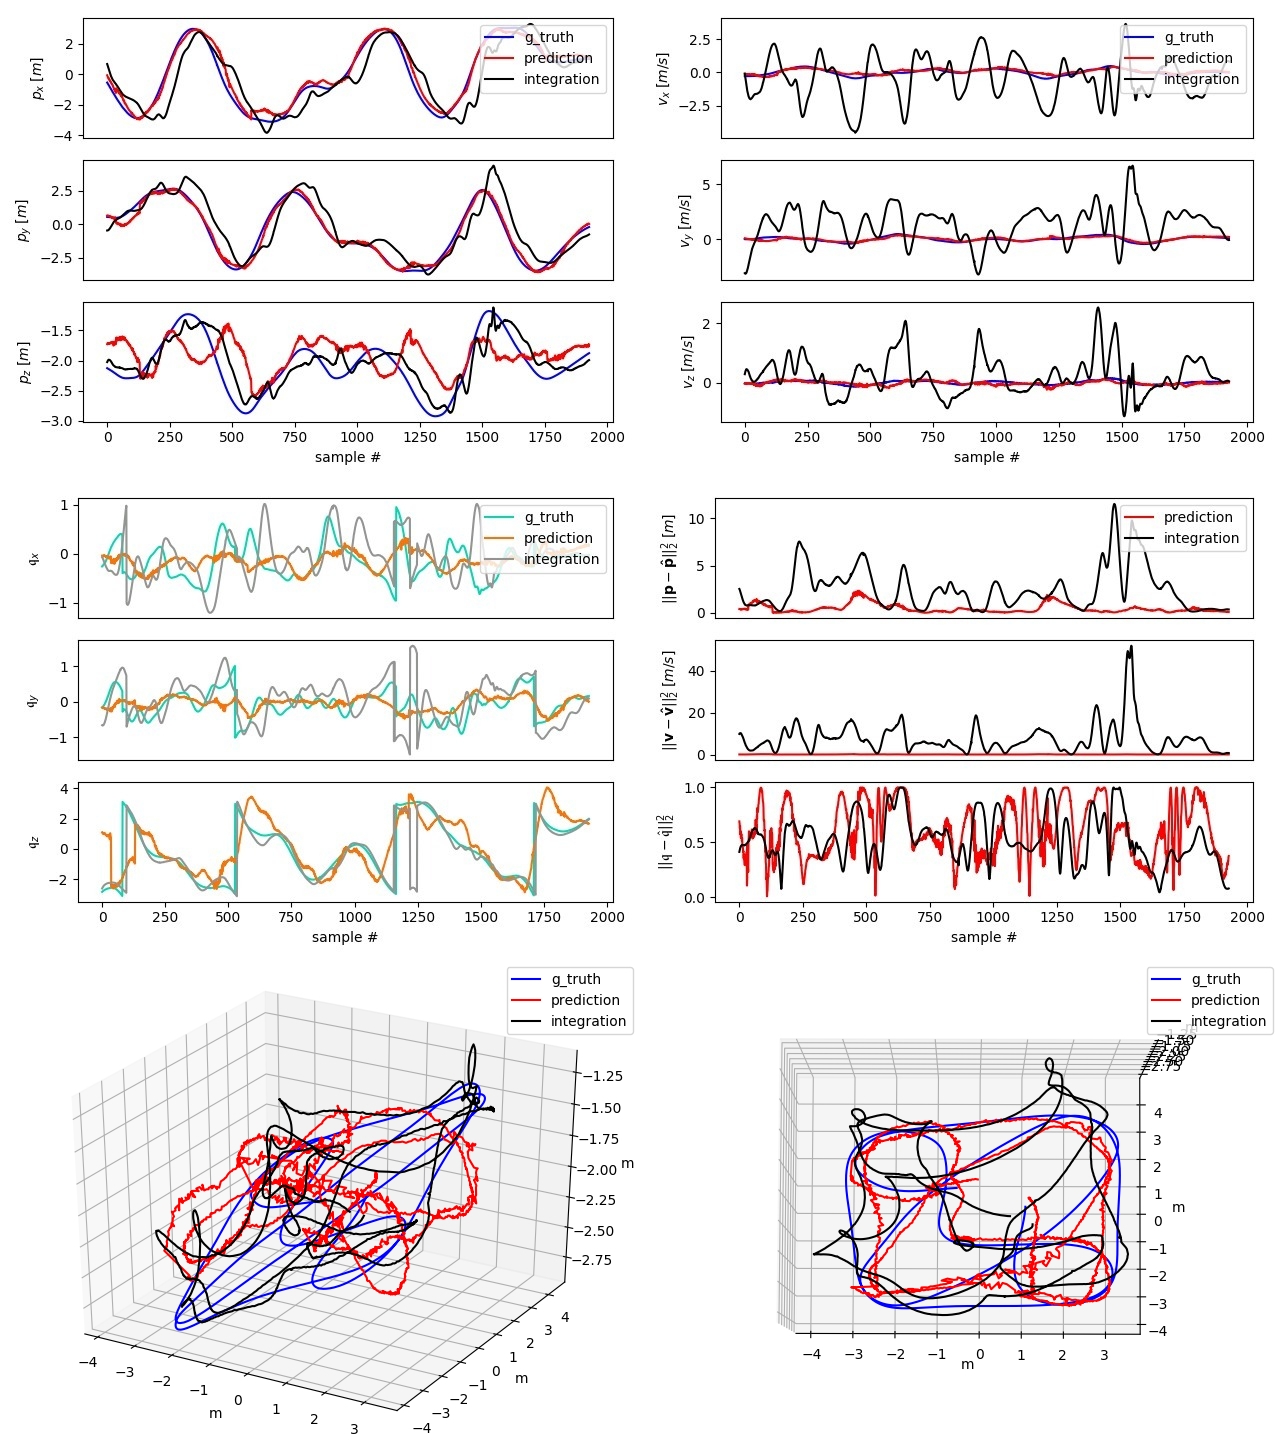
\includegraphics[width=0.85\textwidth]{thesis_template/img/tilted_thrice_so3_full.jpg}
   \caption{Results of the $\mathfrak{so}(3)$-based IMU integration deep model on a fragment of the test sequence \emph{tiltedThrice}@6m/s compared with ground truth and IMU double integration. From left to right, and top to bottom, the plots represent: $\mathbf{p}$, $\mathbf{v}$, $\boldsymbol{\mathfrak{q}}$, the errors wrt. the ground truth, and the 3D views of $\mathbf{p}$.}
   \label{fig:imu_so3_tiltedThrice_val}
\end{figure}

As a sanity check, we perform the \emph{iterative experiment} using both the training set (i.e. with the \emph{bentDice} training sequence), and the \emph{tiltedThrice} test set. 
The aim of this experiment is to see if the model can overcome somehow the noise of the IMU at a longer time span.
In Figure \ref{fig:imu_so3_iterative_bentDice_vs_tiltedThrice_pos} we show the results for the position estimate for both datasets.
We don't show the results for the IMU double integration because they drift significantly more, and they completely distort the view of the plots. 

\begin{figure}[h]
   \centering
   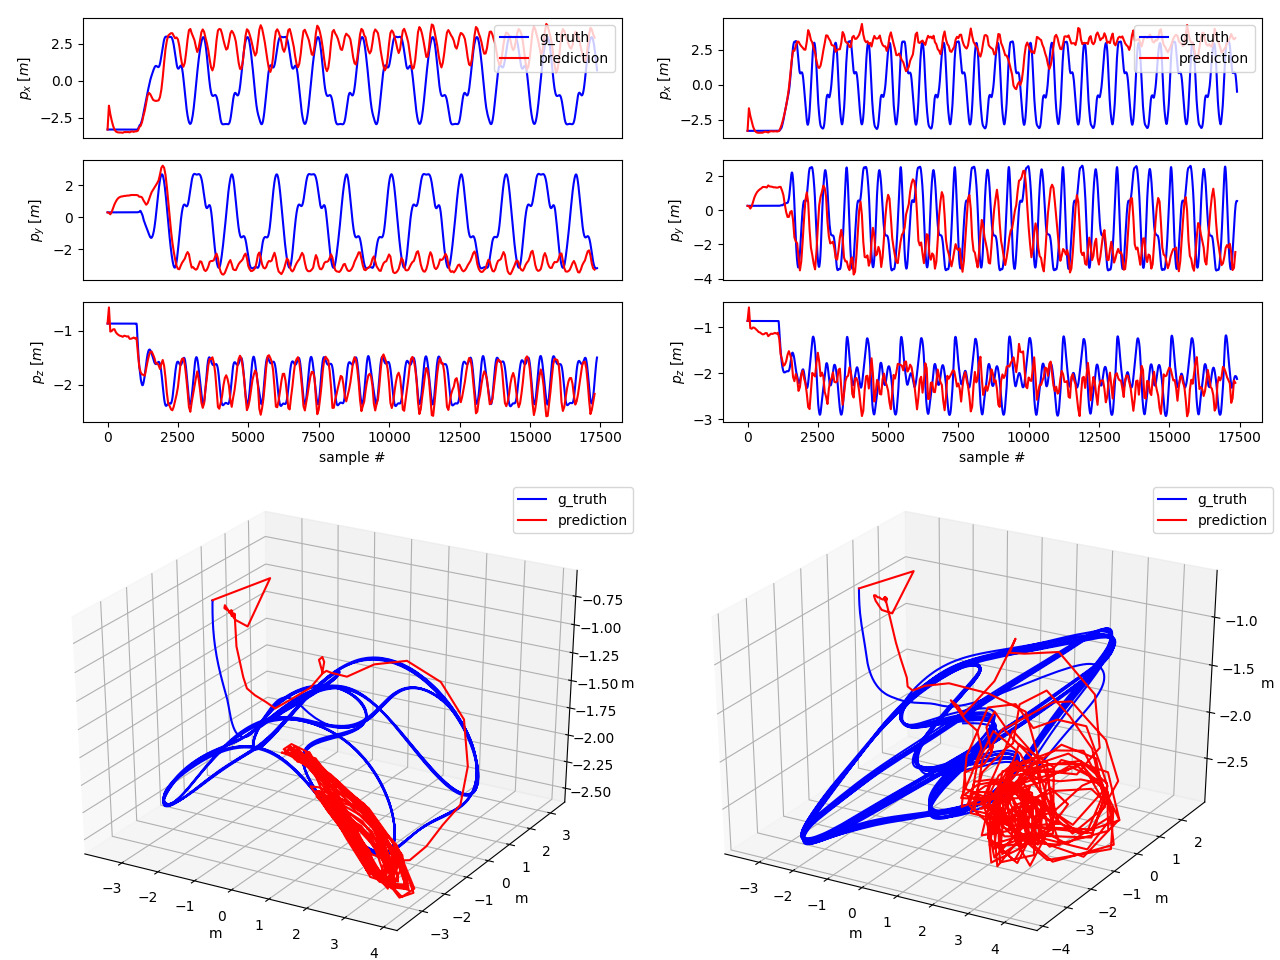
\includegraphics[width=0.85\textwidth]{thesis_template/img/iterative_bentDice_vs_tiltedThrice.jpg}
   \caption{Results of the iterative experiment on both the training set (left column) and test set (right column), using the \emph{bentDice}@2m/s and \emph{tiltedThrice}@6m/s respectively. It can be shown that the model cannot properly follow the trajectory in neither of the cases, although it does not drift to arbitrarily large values.}
   \label{fig:imu_so3_iterative_bentDice_vs_tiltedThrice_pos}
\end{figure}

From Figure \ref{fig:imu_so3_iterative_bentDice_vs_tiltedThrice_pos}, we can see that the model is not quite following the trajectory, and is instead doing some sort of periodic movements for the three output $(\mathbf{\hat{p}}, \mathbf{\hat{v}}, \mathfrak{\hat{q}})^T$. 
This leads to the hypothesis that the model is not really learning proper integration, but some kind of fixed mapping between initial state and final state.
At the end of the day, it is probably the easiest thing to do for a deep model, since both states are quite similar when using a window of $w=50$, which only corresponds to a time uncertainty of 0.5 seconds in the BB dataset. 

To test this hypothesis, and to verify if the architecture of the model makes sense at all, we run the iterative experiment again for the \emph{bentDice} training dataset with four variants. For each of these, we deactivate some connections of the network architecture from Figure \ref{fig:state_int_v0}, and perform inference on the specified dataset. The results of the following four tests are shown in Figure \ref{fig:iterative_bentDice_contributions}:
\begin{enumerate}
    \item\label{item:iterative_no_CNN} In the upper-left plot, we remove the connections from the CNN module in the concatenating layer.
    \item\label{item:iterative_no_IMU_skip} In the upper-right plot, we remove the skip connections from the IMU matrix in the concatenating layer.
    \item\label{item:iterative_just_state_0} In the lower-left plot, we remove all connections except for the initial state.
    \item\label{item:iterative_just_imu_data} In the lower-right plot, we remove the connections of the initial state.
\end{enumerate}

\begin{figure}[h]
   \centering
   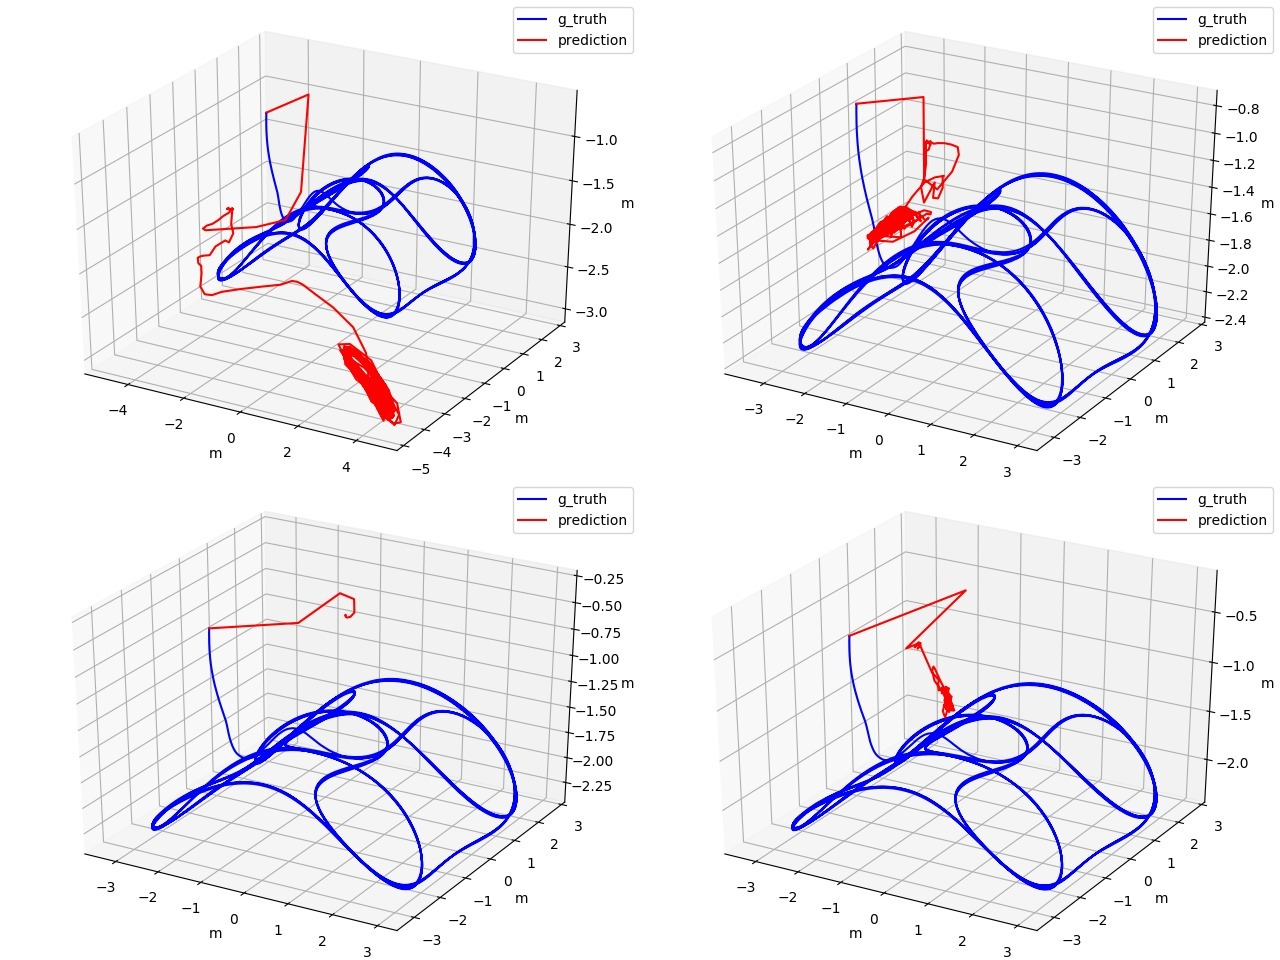
\includegraphics[width=0.85\textwidth]{thesis_template/img/iterative_bentDice_contributions.jpg}
   \caption{Results of the iterative experiment on the training set (\emph{bentDice}@2m/s), where several connections have been disabled in the network. Upper-left: no CNN information. Upper-right: no IMU information. Lower-left: Only initial state information. Lower-right: no initial state information.}
   \label{fig:iterative_bentDice_contributions}
\end{figure}

After accurate analysis of the results shown in Figure \ref{fig:iterative_bentDice_contributions}, we can see that the model is actually learning some sort of IMU integration, in fact. 
In experiment (\ref{item:iterative_just_state_0}.), where only the initial state is being used, we see that there is barely any motion at all
This is what one would expected of IMU integration, because the system should use the IMU data to deduce how the initial state has changed. 
However, for this experiment the IMU data contribution has been completely shortcut, and therefore the state should not be changing. 

On the other hand, in experiment (\ref{item:iterative_just_imu_data}.), which does not have information about the initial state, we can see that in fact there is a lot of small movements around position $(0, 0, -1)^T$.
If the deep model has correctly learned to integrate the IMU data, but has no information about the initial state, then one would indeed expect to see small movements around point $(0, 0, 0)^T$. We can therefore see that the model is actually learning correctly integration in the x and y axes, but it is somehow overfitting the z axis.

Finally, by comparing experiments (\ref{item:iterative_no_CNN}.) and (\ref{item:iterative_no_IMU_skip}.), we can see that most of the unwanted periodic motion comes in fact from the skip connection of the IMU matrix, which probably is distracting the model from learning. 
This means that indeed the convolutional layers may be useful to process the IMU, and extract relevant features for integration. 

\section{Third model: IMU pre-integrator}

The last training approach that we study is what we call the IMU \emph{pre-integrator} (derived in Section \ref{sec:pre_int_training}).
This model is in fact two concatenated models, where only the former is trainable.
It receives as input just the IMU data $\mathbf{\hat{M}}$, from which it is supposed to predict the pre-integration states $(\Delta\mathfrak{\tilde{q}}_{ik}, \Delta\mathbf{\tilde{v}}_{ik}, \Delta\mathbf{\tilde{p}}_{ik})$ derived in \ref{sec:pre_int_training} for all samples $k$ in the time window $[i, i+w]$.
With these pre-integration variables, then the latter model can calculate a prediction for the new state $\mathbf{x}(i+w)$ given $\mathbf{x}(i)$ in a fixed, non-trainable way.

This task proved to be difficult to train for four different reasons.
\begin{itemize}
    \item The number of trainable parameters is quite small (less than 180K).
    \item The output space is large, and larger than the input space. In particular, the model outputs three matrices of dimensions $w\times3$, plus one vector of size $10$. 
    When using $w=50$, this represents a total of $460$ output values, while the input is $300$-dimensional.
    \item There are non-trivial relationships between all the variables in the output space.
    \item The input data cannot be normalized because the scale is important in this problem.
\end{itemize}
Therefore, to be able to properly solve this prediction task, the model is forced to exploit as much as possible the temporal dependence between the variables of the output space by means of a very guided architecture.
Inspired from the literature, we train the model with four different losses: 3 for the pre-integration terms, and one for the state output. 
We derived in Section \ref{sec:pre_int_training}, however, how we can use the fixed nature of the second model to reduce these four losses back to three. 

The model is again trained using the \emph{bentDice} sequence from the Blackbird dataset at a maximum speed of 2m/s, and using an hyperparameter value for the window length of $w=50$.
Following the indications in \cite{DBLP:journals/corr/ClarkWWMT17}, we choose the parameters $a=1$, and $b=0.1$ for our loss function for the first 30 epochs. 
Then, for 20 more epochs, increase $b$ to $0.5$. 
The \emph{one-step} experiment is first performed on a held out part of the \emph{bentDice} flight, and on the harder \emph{tiltedThrice} flight, as with the previous model.
For now, we concentrate on the first three outputs of the model, i.e., the pre-integrated values $(\Delta\mathfrak{\tilde{q}}_{ik}, \Delta\mathbf{\tilde{v}}_{ik}, \Delta\mathbf{\tilde{p}}_{ik})$. The results of this experiment are provided in Figure \ref{fig:pre_integration_original_4loss_bentDice_vs_tiltedThrice}.

\begin{figure}[h]
   \centering
   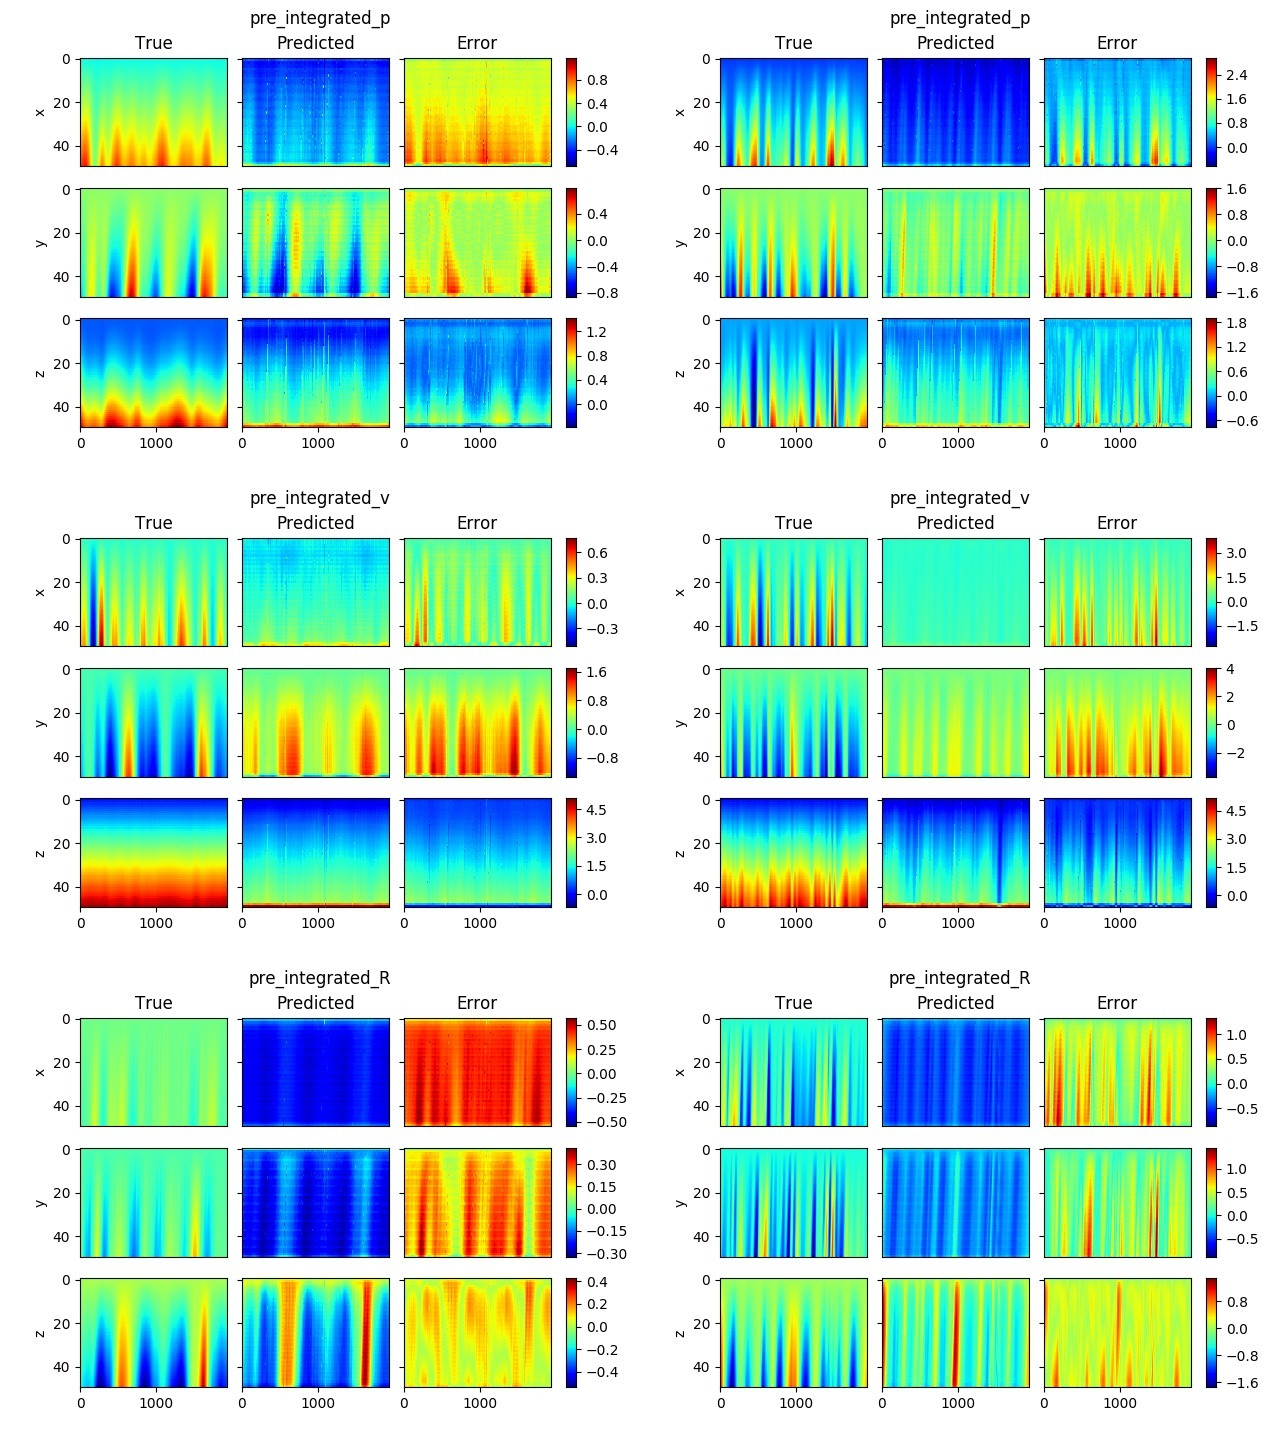
\includegraphics[width=0.85\textwidth]{thesis_template/img/original_4_loss_bentDice_vs_tiltedThrice.jpg}
   \caption{Pre-integration results of the one-step experiment on the validation sets \emph{bentDice}@2m/s (1st column) and \emph{tiltedThrice}@6m/s (2nd column). From top to bottom, rows represent $\Delta\mathbf{\tilde{p}}_{ik}, \Delta\mathbf{\tilde{v}}_{ik}$ and $ \Delta\mathfrak{\tilde{q}}_{ik}$. Inside of each of the 6 plots, the three rows are the x, y, and z components of the specific variable.}
   \label{fig:pre_integration_original_4loss_bentDice_vs_tiltedThrice}
\end{figure}

From Figure \ref{fig:pre_integration_original_4loss_bentDice_vs_tiltedThrice} it is important to understand what each axis in each subplot means.
The horizontal axis still represents the time domain; each column is the output of the model for time sample $k$.
In this case, the input is the window of IMU measurements $\mathbf{\hat{M}}_k$, from $k-w$ until $k$.
Since the pre-integrated variables (model outputs) are $\mathbb{R}^{w\times 3}$ matrices, where the $3$ corresponds to the $(x, y, z)$ components, each output is decomposed into three subplots, where each one has $w$ outputs, sorted as columns.

We can therefore see in Figure \ref{fig:pre_integration_original_4loss_bentDice_vs_tiltedThrice} that indeed the model has a much less error in the last row, which corresponds to the value that is used to compute the output state, and thus receives the 4th loss component.
Although it is important that the model has a low error on this term, the pre-integrated values should be \emph{smooth} vertically.
This sharp discontinuity means that the model has not quite learned the task well. 
Furthermore, we can see that in some cases the predictions do not quite match the ground truth.
We empirically found that a very good way to visually condense all the metrics of the model into a single plot, is to let the model reconstruct the 3D position trajectory.
Since the $\mathbf{\hat{p}}$ value depends on all the variables in the output space, it has a lot of information regarding the general performance. 
The two reconstructed trajectories are shown in Figure \ref{fig:position_3D_original_4loss_bentDice_vs_tiltedThrice}, where it can be seen that the model has trouble especially with the $z$ component of the integration.

\begin{figure}[h]
   \centering
   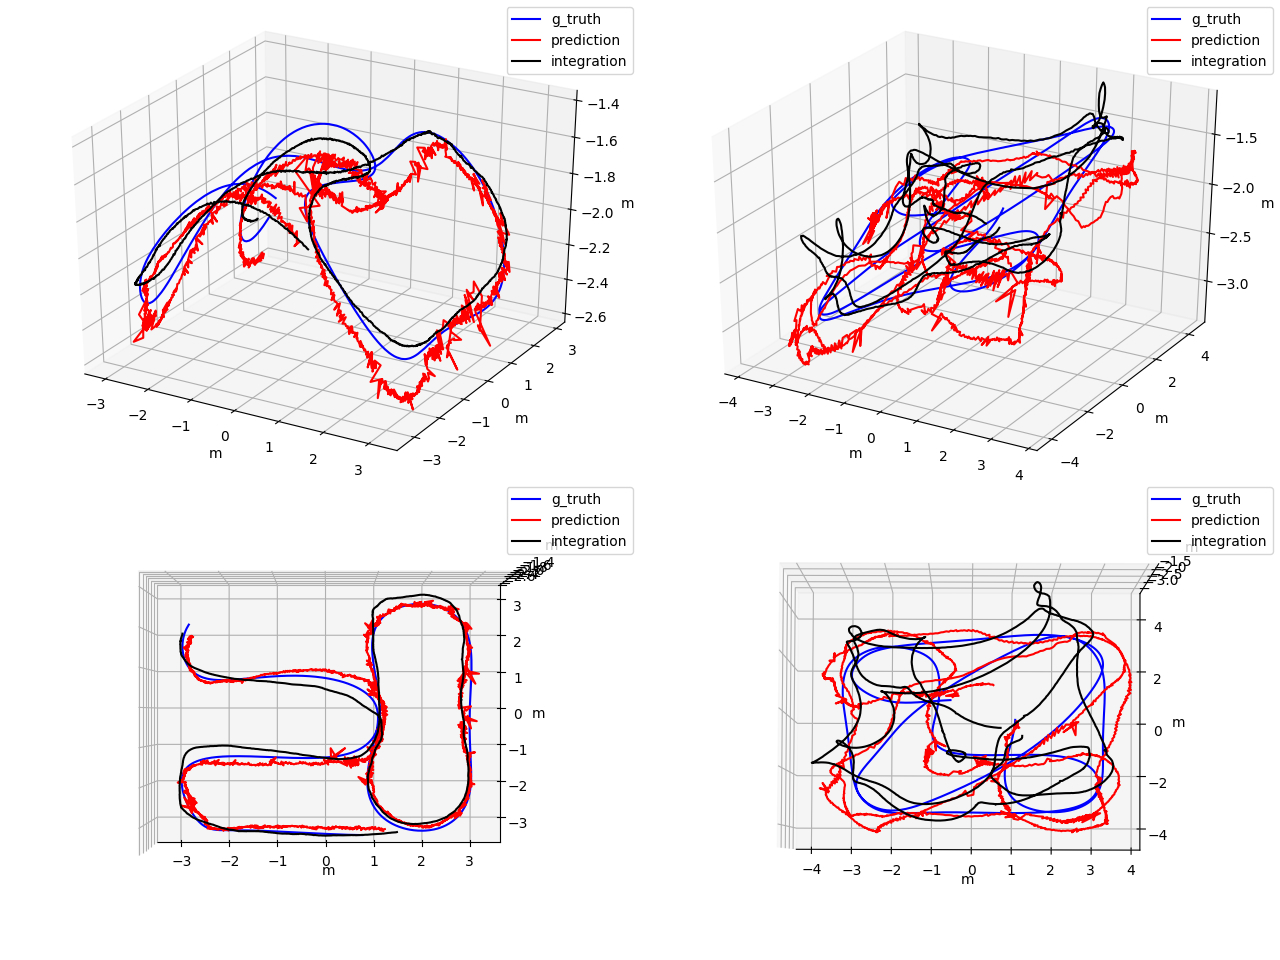
\includegraphics[width=0.85\textwidth]{thesis_template/img/pre_integration_original_4_loss_bentDice_vs_tiltedThrice_3D.jpg}
   \caption{Position vector output of the one-step experiment on the validation sets \emph{bentDice}@2m/s (1st. column) and \emph{tiltedThrice}@6m/s (2nd column).
   The precision of the algorithm in the x and y axes is much higher than in the z axis.}
   \label{fig:position_3D_original_4loss_bentDice_vs_tiltedThrice}
\end{figure}

In an attempt to fix the \emph{smoothness} problem, we introduce two added regularization terms to the training graph.
The first, harshly penalizes if the first row of any pre-integrated value differs from zero.
The second, adds a loss term proportional to the differences between two successive rows in the output, in a sort of way acting as a \emph{diffusion} mechanism along the time ($w$) dimension.
In other words, this latter regularization term penalizes sharp discontinuities in the pre-integrated values, with the aim of enforcing a temporal consistency in the output.
This regularization is weighted by a parameter, which we refer to as $r_\nabla$, which weights the added loss.
Tuning the coefficient of this regularization term proves to be extremely difficult, however, as there are now 6 loss terms in the system.
For instance, an over-tuning of this coefficient yields the results in Figure \ref{fig:position_overtuned_reg_bentDice}, where the network prefers to output zero for almost all the $k$ rows, and right at the end jump to the final value suddenly.
Interestingly, however, we can see that, although clearly being offset, the output is much smoother than in \ref{fig:position_3D_original_4loss_bentDice_vs_tiltedThrice}.

\begin{figure}[h]
   \centering
   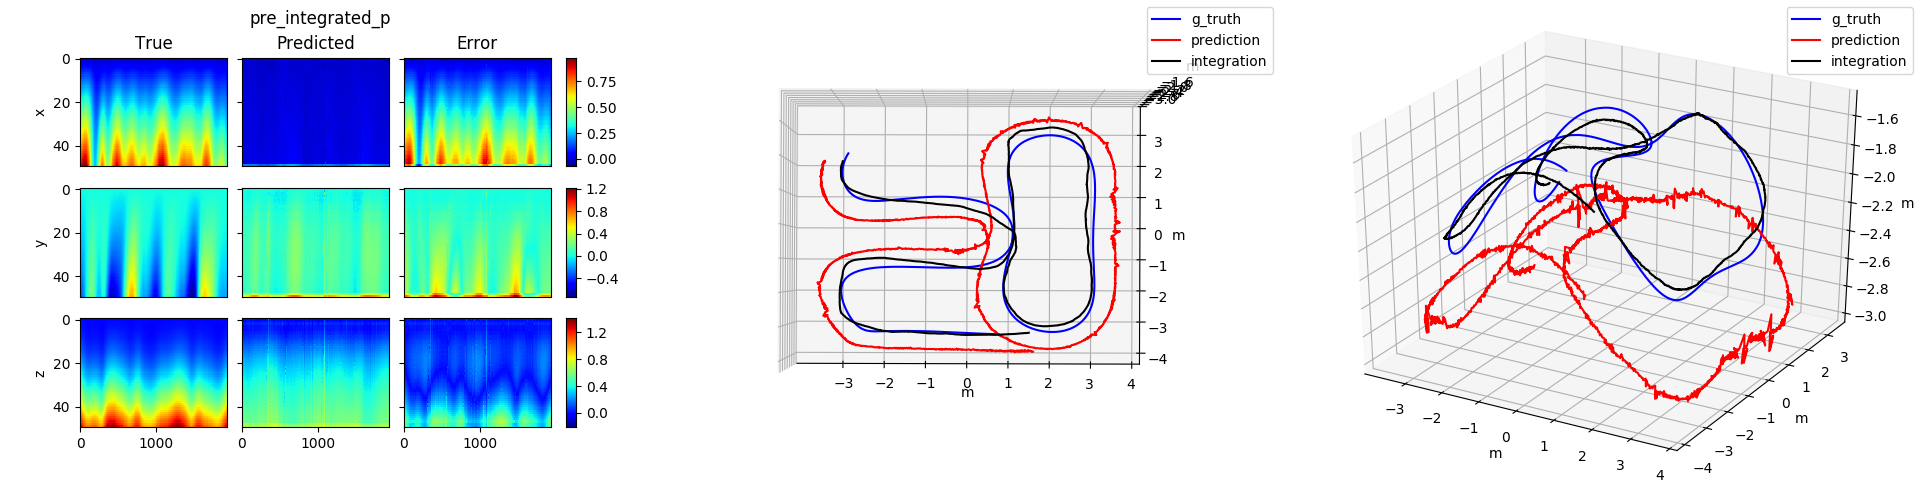
\includegraphics[width=0.95\textwidth]{thesis_template/img/pre_integrated_p_overtuned_results.jpg}
   \caption{Pre-integrated and output position vectors of the one-step experiment on the \emph{bentDice}@2m/s validation set. The \emph{diffusion} regularization term has been over-tuned and the training procedure prioritizes the optimization of this loss factor rather than the actual task loss. 
   This translates into an under-estimated position pre-integration output. 
   However, the results are much more consistent between them than in Figure \ref{fig:position_3D_original_4loss_bentDice_vs_tiltedThrice}.}
   \label{fig:position_overtuned_reg_bentDice}
\end{figure}

After several iterations of trial-and-error, the best parameter combination we find for the loss hyperparameters are: $r_\nabla=0.005$ and $b=0.5$.
With this setup, the we get the results provided in Figure \ref{fig:pre_integration_p3d_best}, on the validation sets \emph{bentDice}@2m/s and \emph{tiltedThrice}@6m/s.
Although we can see in the error plots that the model reasonably outperforms double integration, it is failing to estimate especially the z component of position. 

\begin{figure}[h]
   \centering
   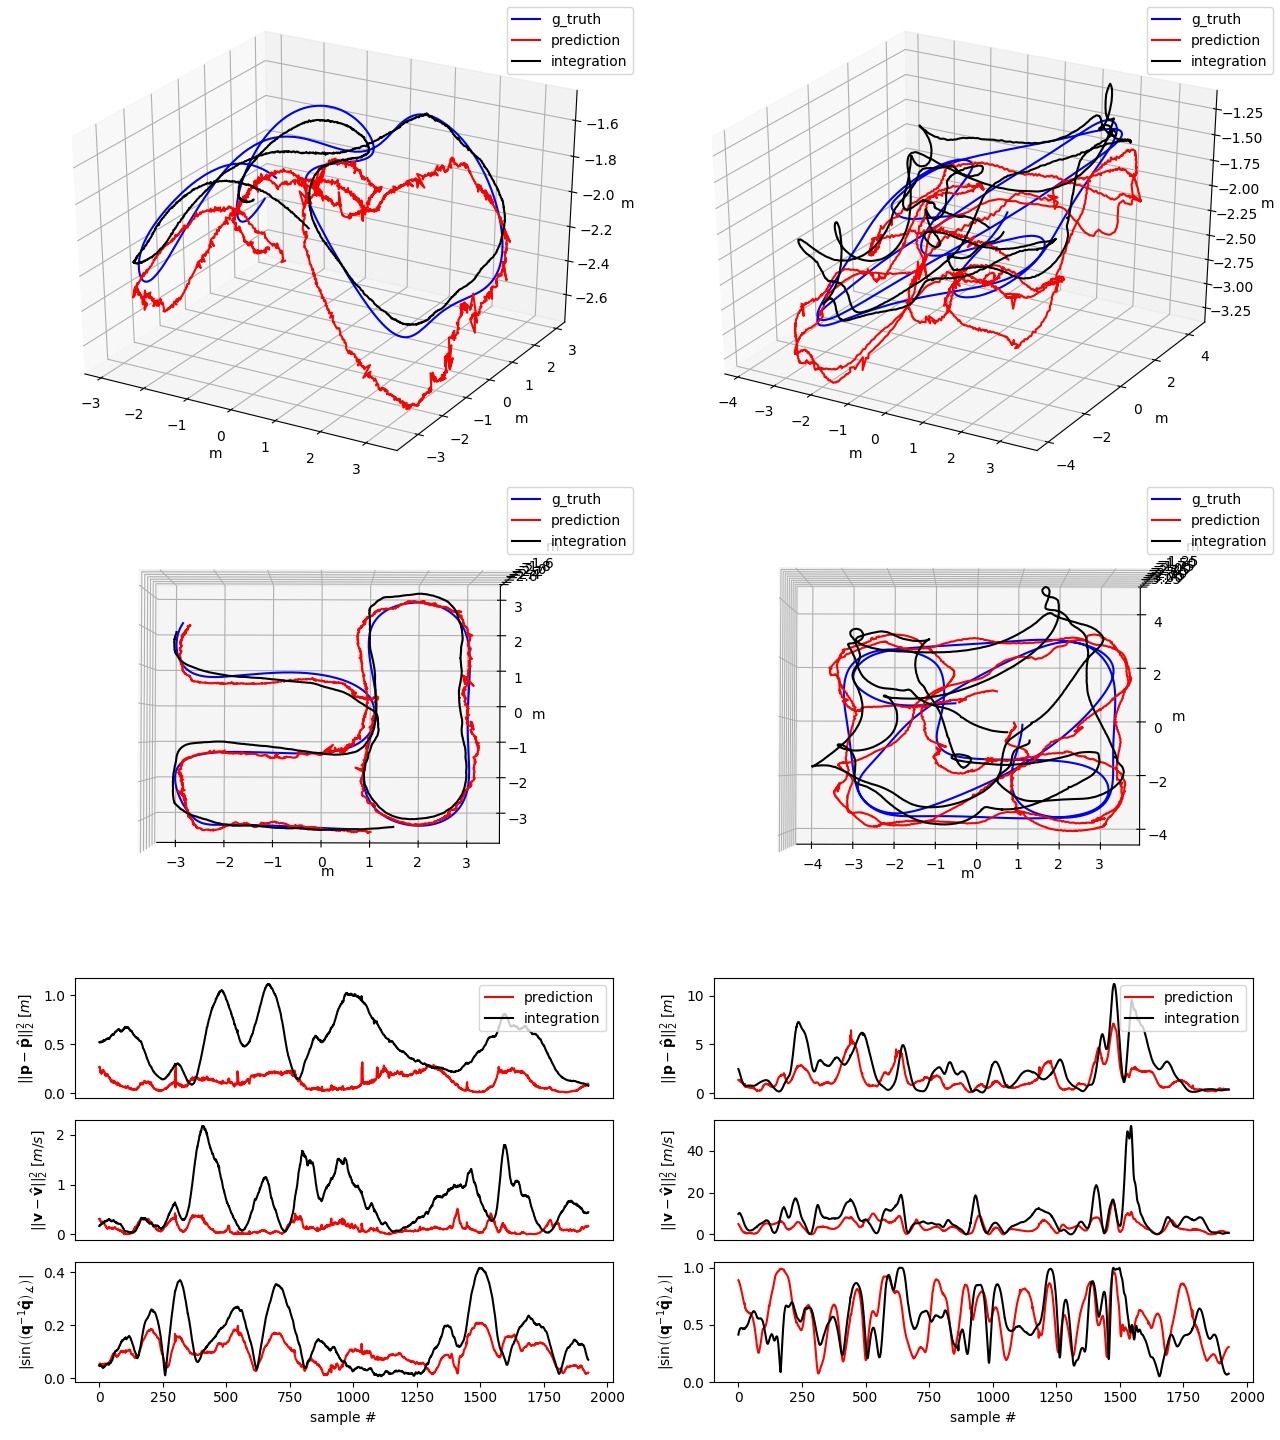
\includegraphics[width=0.95\textwidth]{thesis_template/img/pre_integration_p3d_best.jpg}
   \caption{Position vector output of the one-step experiment on the validation sets \emph{bentDice}@2m/s (1st. column) and \emph{tiltedThrice}@6m/s (2nd column).}
   \label{fig:pre_integration_p3d_best}
\end{figure}

If we perform instead the \emph{iterative} experiment with this last version of the trained model, we verify that this model is not able to compensate the drift (see Figure \ref{fig:pre_integration_iterative_validation}), although it manages to reduce it when compared to IMU integration, both in the position and velocity estimates.
It is difficult to assess whether the rotation estimate is better or worse in the predicted case compared to the integrated one.

\begin{figure}[h]
   \centering
   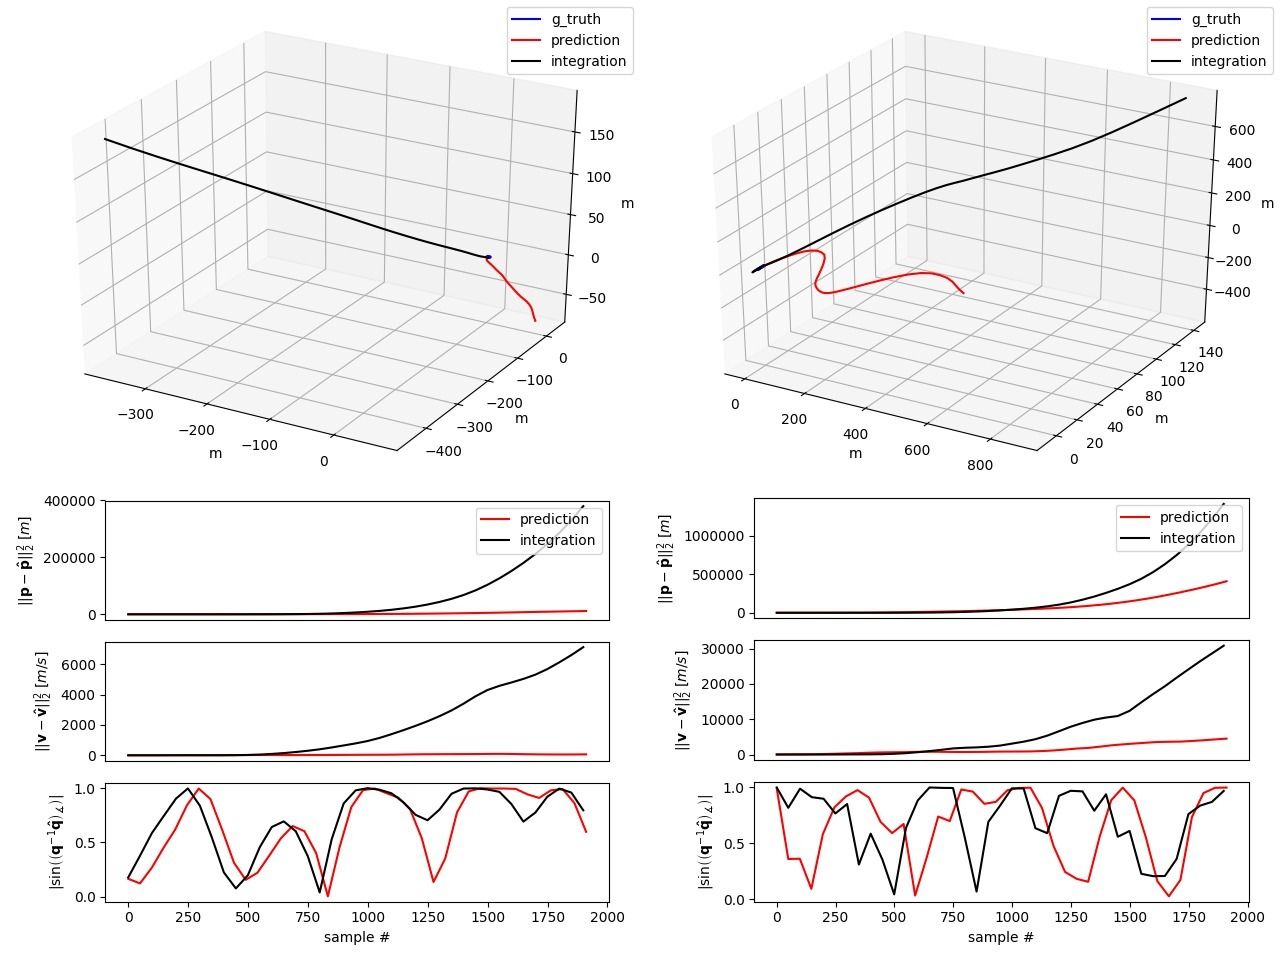
\includegraphics[width=0.95\textwidth]{thesis_template/img/iterative_experiment_pre_integration_pos.jpg}
   \caption{Position vector output of the iterative experiment on the validation sets \emph{bentDice}@2m/s (1st. column) and \emph{tiltedThrice}@6m/s (2nd column).}
   \label{fig:pre_integration_iterative_validation}
\end{figure}

\section{General comparison}

As a wrap-up of the results so far, we run both the one-step and iterative tests for the three available versions of IMU integration deep models.
These three are the two versions of the normal integrator model from Section \ref{sec:imu_state_int} (with quaternion and $\mathfrak{so}(3)$ rotation representation) and the proposed pre-integration model from Section \ref{sec:pre_int_training}.
Also, for each experiment, three datasets are used.
The first is the training dataset, which is a long sequence used for training the models (the first 90\% of the \emph{bentDice}@2m/s dataset). 
The second is the remaining kept-aside 10\% of the training dataset, labeled as test easy (E).
Finally the last is a short sequence of the same length as test (E) from the much harder (H) set \emph{tiltedThrice}@6m/s.
The error terms of the three model predictions are computed from the ground truth data by computing the squared l2 norm, and the average value over the entire used sequence is obtained. 
The results of these experiments are summarized in Table \ref{table:model_comparisons}.

\begin{table}[]
\begin{tabular}{c|c|ccc|ccc|}
\cline{3-8}
\multicolumn{2}{c|}{\multirow{3}{*}{}}                           & \multicolumn{6}{c|}{\textbf{experiment}}                                                                                                                                          \\ \cline{3-8} 
\multicolumn{2}{c|}{}                                            & \multicolumn{3}{c|}{one-step}                                               & \multicolumn{3}{c|}{iterative}                                                             \\ \cline{3-8} 
\multicolumn{2}{c|}{}                                            & \multicolumn{1}{c|}{train} & \multicolumn{1}{c|}{test (E)} & test (H)       & \multicolumn{1}{c|}{train} & \multicolumn{1}{c|}{test (E)} & \multicolumn{1}{c|}{test (H)} \\ \hline
\multicolumn{1}{|c|}{\multirow{4}{*}{\rotatebox[origin=c]{90}{$\left\|\mathbf{p}^e\right\|_2^2$\;[m]}}}   & int     & 0.675                      & 0.644                         & 1.067          & 6.035                     & 5.550                        & 5.809                        \\
\multicolumn{1}{|c|}{}                                & $\mathfrak{so}(3)$     & \textbf{0.179}             & \textbf{0.182}                & \textbf{0.669} & \textbf{4.431}            & \textbf{4.215}               & \textbf{4.502}               \\
\multicolumn{1}{|c|}{}                                & pre-int     & 0.359                      & 0.344                         & 1.234          & 5.7e3                      & 50.990                         & 2.9e2                         \\
\multicolumn{1}{|c|}{}                                & IMU 2int & 0.713                      & 0.731                         & 1.583          & 1.8e4                      & 2.5e2                         & 4.7e2                         \\ \hline
\multicolumn{1}{|c|}{\multirow{4}{*}{\rotatebox[origin=c]{90}{$\left\|\mathbf{v}^e\right\|_2^2\;\left[\frac{m}{s}\right]$}}} & int     & 0.100                      & 0.122                         & 0.217          & 0.249                      & 0.257                         & \textbf{0.350}                \\
\multicolumn{1}{|c|}{}                                & $\mathfrak{so}(3)$     & \textbf{0.071}             & \textbf{0.077}                & \textbf{0.182} & \textbf{0.184}             & \textbf{0.219}                & 0.424                         \\
\multicolumn{1}{|c|}{}                                & pre-int     & 0.370                      & 0.356                         & 1.933          & 2.8e2                      & 6.170                        & 38.730                         \\
\multicolumn{1}{|c|}{}                                & IMU 2int & 0.826                      & 0.810                         & 2.727          & 2.9e2                      & 43.589                         & 84.853                         \\ \hline
\multicolumn{1}{|c|}{\multirow{4}{*}{\rotatebox[origin=c]{90}{$\sin\mathbf{q}^e_\measuredangle$[rad]}}}       & int     & 0.482                      & 0.433                         & 0.619          & \textbf{0.540}             & \textbf{0.282}                & \textbf{0.129}                \\
\multicolumn{1}{|c|}{}                                & $\mathfrak{so}(3)$     & 0.252                      & 0.274                         & 0.612          & 0.574                      & 0.591                         & 0.676                         \\
\multicolumn{1}{|c|}{}                                & pre-int     & \textbf{0.086}            & \textbf{0.097}                & 0.563          & 0.642                      & 0.655                         & 0.657                         \\
\multicolumn{1}{|c|}{}                                & IMU 2int & 0.121                      & 0.148                         & \textbf{0.533} & 0.644                      & 0.710                         & 0.708                         \\ \hline
\end{tabular}
\captionof{table}{Performance comparison of the three IMU integration models with vanilla double integration.
The errors are computed with the loss functions described by \ref{eq:q_state_loss} with the ground truth data.
The models are tested on the long training set, an two shorter test sets, labeled as easy (E) and hard (H).
The easy test set is a held-out test set from \emph{bentDice}@2m/s and the hard set is a fragment of \emph{tiltedThrice}@6m/s, of the same length as the easy test set.
Results show that $\mathfrak{so}(3)$-based integration model outperforms the rest on nearly all experiments for both position and velocity estimation. 
The best rotation results are much more inhomogeneous.
    \label{table:model_comparisons}}
\end{table}

An analysis of such table shows that the $\mathfrak{so}(3)$-based state integrating model outperforms the rest in almost all cases for the position and velocity estimates.
More particularly, it achieves an error for position in the difficult test set in the one-step integration experiment of $\sqrt{0.448}=0.67m$, which is significantly lower than in the other cases.
It also behaves much better than the other models in the iterative experiment, because as we saw in Figures \ref{fig:imu_so3_bentdice_val} and \ref{fig:imu_so3_tiltedThrice_val}, the estimate does not drift away from the span of the input data.
This, however, does not really mean that its predictions are good for this case, as it can also be seen in the same two figures.
Unfortunately, the metrics for the rotation prediction are not very reliable for determining which model performs better or worse at this case, as the error cannot be defined in an euclidean way.
In fact, no matter if we use Lie Algebra or quaternions as rotation base, the rotation error is periodic, and therefore especially in the iterative case, the metrics are not very useful to actually infer the performance of the model.
However, for the one-step experiment, where rotations are small enough for not going through sign flips in one window, it looks like indeed the $\mathfrak{so}(3)$ formulations of the second and third models help to learn better the rotation term.

